\documentclass[11pt,compress,t,notes=noshow, aspectratio=169, xcolor=table]{beamer}

\usepackage{../../style/lmu-lecture}
% Defines macros and environments
% This file is included in slides and exercises

% Rarely used fontstyle for R packages, used only in 
% - forests/slides-forests-benchmark.tex
% - exercises/single-exercises/methods_l_1.Rnw
% - slides/cart/attic/slides_extra_trees.Rnw
\newcommand{\pkg}[1]{{\fontseries{b}\selectfont #1}}

% Spacing helpers, used often (mostly in exercises for \dlz)
\newcommand{\lz}{\vspace{0.5cm}} % vertical space (used often in slides)
\newcommand{\dlz}{\vspace{1cm}}  % double vertical space (used often in exercises, never in slides)
\newcommand{\oneliner}[1] % Oneliner for important statements, used e.g. in iml, algods
{\begin{block}{}\begin{center}\begin{Large}#1\end{Large}\end{center}\end{block}}

% Don't know if this is used or needed, remove?
% textcolor that works in mathmode
% https://tex.stackexchange.com/a/261480
% Used e.g. in forests/slides-forests-bagging.tex
% [...] \textcolor{blue}{\tfrac{1}{M}\sum^M_{m} [...]
% \makeatletter
% \renewcommand*{\@textcolor}[3]{%
%   \protect\leavevmode
%   \begingroup
%     \color#1{#2}#3%
%   \endgroup
% }
% \makeatother




\title{Interpretable Machine Learning}
% \author{LMU}
%\institute{\href{https://compstat-lmu.github.io/lecture_iml/}{compstat-lmu.github.io/lecture\_iml}}
\date{}

%\bibliography{feature-importance}
%\usepackage{Sweave}
\begin{document}
	\newcommand{\titlefigure}{figure_man/pimp}
    \newcommand{\learninggoals}{
    	\item Understand PIMP and its motivation
            \item Address multiple testing in feature importance}
	% Set style/preamble.Rnw as parent.
	
	% Load all R packages and set up knitr
	
	% This file loads R packages, configures knitr options and sets preamble.Rnw as 
	% parent file
	% IF YOU MODIFY THIS, PLZ ALSO MODIFY setup.Rmd ACCORDINGLY...
	
	% Defines macros and environments

	\lecturechapter{PIMP}
	\lecture{Interpretable Machine Learning}
	
	% ------------------------------------------------------------------------------


\begin{frame}{Testing Importance (PIMP) \citebutton{Altmann et al. (2010)}{https://doi.org/10.1093/bioinformatics/btq134}}

\begin{itemize}[<+->]
  \item PIMP was originally introduced for random forest's built-in PFI scores
  %\item It fixes the problem that the importance measure prefers features with many categories.
  \item PIMP idea: Test if an observed $\widehat{\text{PFI}}_j^{\text{obs}}$ score is \emph{significantly} greater than expected under the null hypothesis of $X_j$ being not important\\
  $\leadsto$ Accounts for spurious importance due to randomness
  %Addresses random fluctuations that cause non-zero PFI scores
  %Useful because PFI can be non-zero due to randomness/stochasticity
  %It computes the distribution of importances under the $H_0$-hypothesis that the feature is independent of the target $y$
 \item Null hypothesis $H_0$: Feature $X_j$ is conditionally independent of $y$ (unimportant)
  \item Approximate null distribution of PFI scores under $H_0$ by repeated permutations:\\
  Permute $y$ $\rightarrow$ retrain model $\rightarrow$ recompute $\widehat{\text{PFI}}_j$ scores for all $j$ $\rightarrow$ repeat $B$ times\\
  $\Rightarrow$ Permuting $y$ breaks relationship to all features (PFI scores reflect noise only)%\\
  %$\Rightarrow$ By computing PFI scores again, we obtain distribution of PFI scores under $H_0$
  \item %We now rescale the importance to a 
  Assess the significance of PFI scores via tail probability under $H_0$\\
  %Compute p-value via tail probability under $H_0$ over all $B$ repetitions
    $\Rightarrow$ Use this as a new feature importance score, adjusting for random chance
  %and use this as new importance measure
\end{itemize}

%\footnote[frame]{\fullcite{altmann2010permutation}}
%{\tiny{Altmann, André, et al. "Permutation importance: a corrected feature importance measure." 
%Bioinformatics 26.10 (2010): 1340-134.}}

\end{frame}

\begin{frame}{PIMP algorithm}

\begin{enumerate}
	\item<1-3> For $b \in \{1, \ldots, B\}$:
		\begin{itemize}
			\item Permute response vector $\yv$, denote permuted target as $\yv^{(b)}$
			\item Retrain model on data $(\Xmat, \yv^{(b)})$ with permuted target 
			\item Compute feature importance $\widehat{\text{PFI}}_j^{(b)}$ for each feature $j$ (under $H_0$)
		\end{itemize}
	\item<2-3> Train model on original data  $(\Xmat, \yv)$ with unpermuted target
	\item<3> For each feature $j \in \{1,\ldots,p\}$:
		\begin{itemize}
        		\item Compute $\widehat{\text{PFI}}_j^{\text{obs}}$ for the model without permutation of $y$ (under $H_1$)
			\item Fit probability distribution to all PFI scores $\{\widehat{\text{PFI}}_j^{(b)}\}_{b=1}^{B}$ (under $H_0$)\\
            e.g., by assuming Gaussian/lognormal/gamma distribution (parametric)%\\
            %$\leadsto$ non-parametric by computing empirical tail probability
			\item Compute p-value: Probability that null importance exceeds observed: 
            \begin{itemize}
                \item parametric by taking tail probability of assumed distribution $$\mathbb{P}(\widehat{\text{PFI}}_j^{(m)} \geq \widehat{\text{PFI}}_j^{\text{obs}})$$
                \item non-parametric by computing empirical tail probability: 
                $$p_j := \tfrac{1}{B} \textstyle \sum_{b=1}^{B} \mathbb{I}[\widehat{\text{PFI}}_j^{(b)} \geq \widehat{\text{PFI}}_j^{\text{obs}}]$$
            \end{itemize}

		\end{itemize}
\end{enumerate}
\end{frame}



%TODO: Simplify or better explain example
\begin{frame}{PIMP for extrapolation example}
\textbf{Recall:} 
 Let $y = x_3 + \epsilon_y$, with $\epsilon_y \sim \mathcal{N}(0, 0.1)$.

\begin{itemize}
  \item $x_1 := \epsilon_1$, $x_2 := x_1 + \epsilon_2$ are highly correlated  
        ($\epsilon_1 \sim \mathcal{N}(0,1)$, $\epsilon_2 \sim \mathcal{N}(0, 0.01)$)
  \item $x_3 := \epsilon_3$, $x_4 := \epsilon_4$, with $\epsilon_3, \epsilon_4 \sim \mathcal{N}(0,1)$ and all noise terms $\epsilon_j$ are independent
  \item Fitting a linear model yields $\hat{f}(\xv) \approx 0.3 x_1 - 0.3 x_2 + x_3$
\end{itemize}

% $y = x_3 + \epsilon_y$ with $\epsilon_y \sim N(0, 0.1)$, 
% $x_1$, $x_2$ highly correlated but independent of $y$, 
% $x_4$ is independent of $y$ and all other variables.
% Fitting a LM yields $\fh(\xv) \approx 0.3 x_1 - 0.3 x_2 + x_3$.
%Fitting a \texttt{lm} yields $\fh(x) \approx 0.3 x_1 - 0.3 x_2 + x_3$.
%
%\begin{figure}
  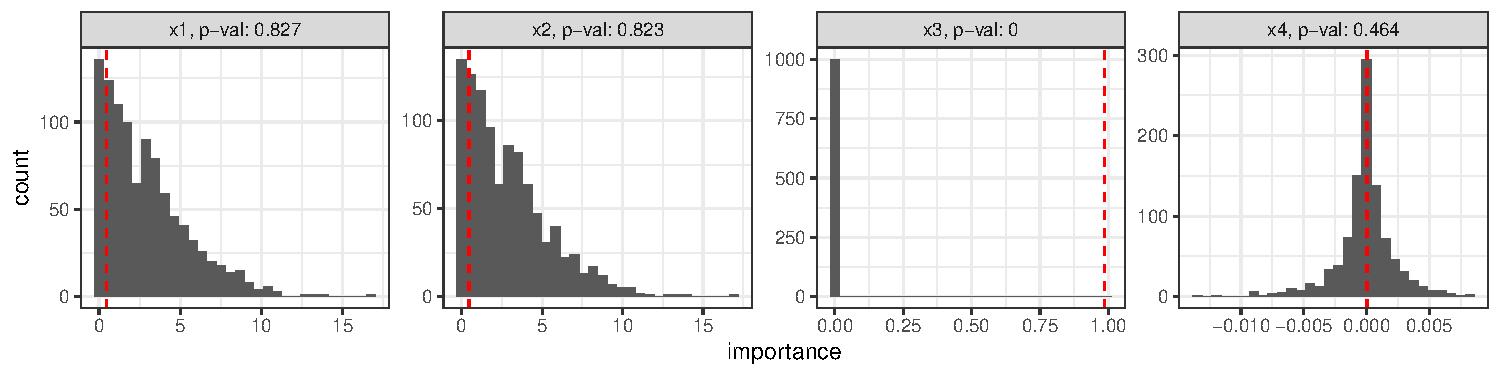
\includegraphics[width=\linewidth]{figure_man/pimp.pdf}
  %\caption{$H_0$ distribution (1000 samples) for each feature as histograms, the true PFI indicated in red. PIMP only considers $x_3$ relevant. Although PFI for $x_1$ and $x_2$ is nonzero, PIMP considers them irrelevant since they are not predictive of $y$. Even after permuting $y$, the model relies on them.}
%\end{figure}

\begin{itemize}
    \item Histograms: $H_0$ distribution of PFI scores after permuting $y$ (1000 repetitions)
    \item Red: Observed PFI score (under $H_1$) $\leadsto$ compare against $H_0$ distribution
    \item Recall: PFI for $x_1$, $x_2$, $x_3$ is nonzero suggesting they are important (red lines)
    \item PIMP considers $x_1$, $x_2$ not significantly relevant (p-value > 0.05) 

    %since they are not predictive of $y$
\end{itemize}
\end{frame}

% \begin{frame}{Digression: Multiple testing problem \citebutton{Romano et al. (2010)}{https://doi.org/10.1057/978-1-349-95121-5_2914-1}}
% \begin{itemize}[<+->]
%   \item When should we reject the $H_0$-hypothesis for a feature? 
%   \item The larger the number of features, the more tests need to be performed by PIMP\\
%   $\leadsto$ \textbf{Multiple testing problem}: If multiplicity of tests is not taken into account, the probability that some of the true $H_0$-hypothesis is rejected (type-I error) by chance may be large
%   \item Accounting for multiplicity of individual tests can be achieved by controlling an appropriate error rate, e.g., the \textbf{family-wise error rate} (FWE: probability of at least one type-I error)
%   \item One classical method to control the FWE is the \textbf{Bonferroni correction} which rejects a null hypothesis if its p-value is smaller than $\alpha/m$ with $m$ as the number of performed parallel tests
%   %\item We refer to other lectures or the statistics literature for more details
%   \end{itemize} 

%   %\footnote[frame]{\fullcite{romano2010multiple}}
%   %{\tiny{Romano, J. P., Shaikh, A. M., and Wolf, M. (2010). Multiple Testing. The New Palgrave Dictionary of Economys. \url{https://home.uchicago.edu/~amshaikh/webfiles/palgrave.pdf}}\par}
% \end{frame}

\begin{frame}{Digression: Multiple Testing \citebutton{Romano et al. (2010)}{https://doi.org/10.1057/978-1-349-95121-5_2914-1}}

\begin{itemize}%[<+->]
  \item When should we reject $H_0$ for a given feature?
  \item PIMP conducts one hypothesis test per feature $\Rightarrow$ \textbf{multiple testing problem}
  \item With many tests, rejections of true $H_0$ just by chance (type-I errors) accumulate
  \item To account for this, control a suitable error rate, e.g., the \textbf{family-wise error rate}\\
  FWE: probability of making at least one type-I error across all tests
  \item A classical method is the \textbf{Bonferroni correction}:\\
  reject $H_0$ if p-value $< \alpha/m$ 
  where $m$ is the number of tests
\end{itemize}

\end{frame}

% \begin{frame}
%   \printbibliography
% \end{frame}

\endlecture
\end{document}
